% !TeX root = ../main.tex

\chapter{Design}
\label{ch:design}

This chapter presents the design of the proposed tiered compilation architecture. Section~\ref{sec:design:overview} introduces the three components---tier-1 baseline JIT, tier-2 selective recompilation, and on-stack replacement---and the pipeline that connects them. Section~\ref{sec:design:context} defines the shared runtime context and the calling conventions that bridge the two compilation tiers. Section~\ref{sec:design:tier1} describes the tier-1 baseline JIT and its embedded profile counters. Section~\ref{sec:design:tier2} describes tier-2 selective recompilation. Section~\ref{sec:design:osr} describes on-stack replacement. The presentation focuses on the design choices that distinguish each mechanism. Pseudocode and algorithm blocks supplement the prose where a mechanism's structure is non-obvious.

\section{Architecture Overview}
\label{sec:design:overview}

The proposed architecture has three components. A lightweight baseline JIT compiles every wasm function at module instantiation. The resulting tier-1 native code runs on the user thread with embedded profile counters. A background worker thread selectively recompiles hot functions through the existing WasmEdge LLVM frontend.

Two promotion paths target the two invocation shapes that matter. The first, function-entry tier-2 promotion, redirects future calls to a hot function into LLVM-compiled code by atomically replacing the function's entry in the dispatch table. The second, on-stack replacement, migrates a currently-executing tier-1 frame into LLVM-compiled code mid-loop, so the in-flight invocation also benefits from optimization. Figure~\ref{fig:design:arch} summarizes the architecture.

\begin{figure}[htbp]
\centering
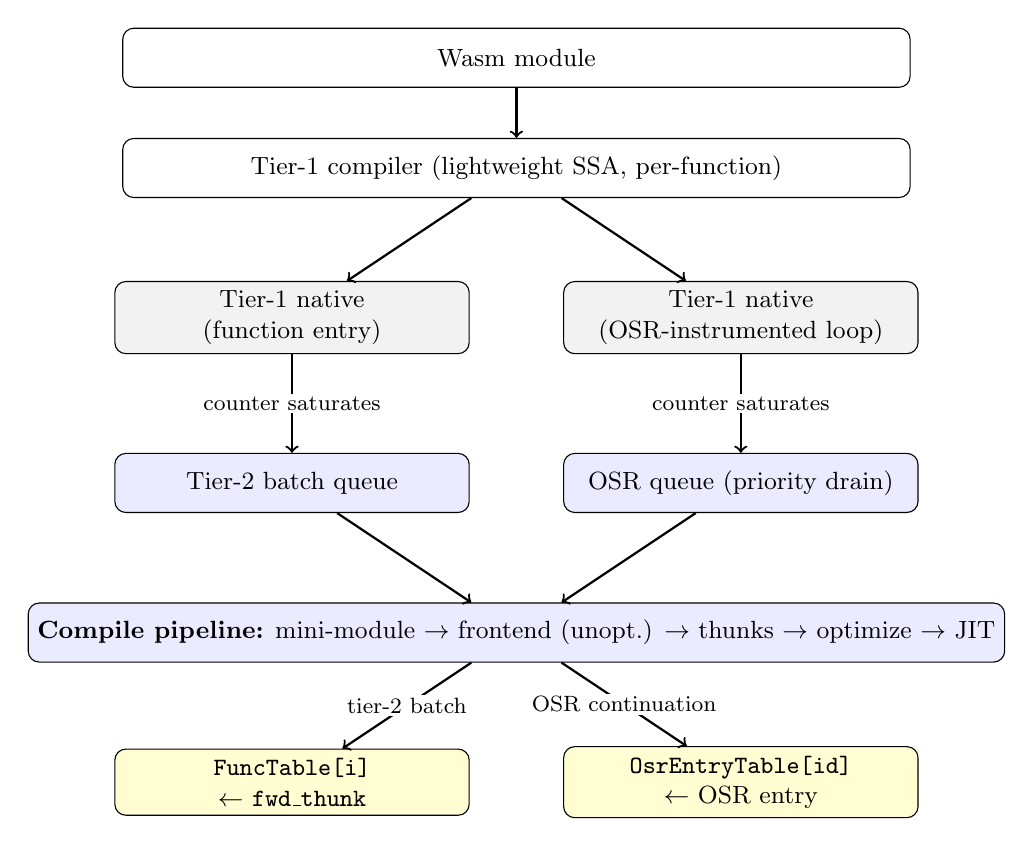
\begin{tikzpicture}[
  font=\small,
  box/.style={draw, rectangle, rounded corners, minimum width=4.5cm, minimum height=0.75cm, align=center},
  wide/.style={draw, rectangle, rounded corners, minimum width=10cm, minimum height=0.75cm, align=center},
  user/.style={fill=gray!10},
  worker/.style={fill=blue!8},
  table/.style={fill=yellow!18},
  arrow/.style={->, thick},
  elabel/.style={font=\footnotesize, fill=white, inner sep=1pt},
]
\node[wide] (input) at (0, 9.0) {Wasm module};
\node[wide] (t1c)   at (0, 7.6) {Tier-1 compiler (lightweight SSA, per-function)};
\node[box, user] (entry) at (-2.85, 5.7) {Tier-1 native\\(function entry)};
\node[box, user] (loop)  at ( 2.85, 5.7) {Tier-1 native\\(OSR-instrumented loop)};
\node[box, worker] (q1) at (-2.85, 3.6) {Tier-2 batch queue};
\node[box, worker] (q2) at ( 2.85, 3.6) {OSR queue (priority drain)};
\node[wide, worker] (pipe) at (0, 1.7) {\textbf{Compile pipeline:} mini-module $\to$ frontend (unopt.) $\to$ thunks $\to$ optimize $\to$ JIT};
\node[box, table] (ftbl) at (-2.85, -0.2) {\texttt{FuncTable[i]}\\$\leftarrow$ \texttt{fwd\_thunk}};
\node[box, table] (otbl) at ( 2.85, -0.2) {\texttt{OsrEntryTable[id]}\\$\leftarrow$ OSR entry};

\draw[arrow] (input) -- (t1c);
\draw[arrow] (t1c) -- (entry);
\draw[arrow] (t1c) -- (loop);
\draw[arrow] (entry) -- node[elabel] {counter saturates} (q1);
\draw[arrow] (loop)  -- node[elabel] {counter saturates} (q2);
\draw[arrow] (q1) -- (pipe);
\draw[arrow] (q2) -- (pipe);
\draw[arrow] (pipe) -- node[elabel] {tier-2 batch} (ftbl);
\draw[arrow] (pipe) -- node[elabel] {OSR continuation} (otbl);
\end{tikzpicture}
\caption{Architecture of the proposed tiered compilation system. The tier-1 compiler (top) lowers every defined function at module instantiation. Tier-1 native code (gray) executes on the user thread and embeds two classes of profile counter. On counter saturation, one of two notifications fires and enqueues a compile request on the tier-2 worker (blue), which drains the OSR queue first and executes a single shared compile pipeline. The result publishes atomically into one of two shared slots (yellow): the \texttt{FuncTable} for function-entry promotion, the \texttt{OsrEntryTable} for OSR.}
\label{fig:design:arch}
\end{figure}

Figure~\ref{fig:design:arch} walks through the five stages of the pipeline. The first three execute on the user thread at module load and during execution; the last two execute asynchronously on the tier-2 worker thread when a profile counter saturates.

The proposed pipeline coexists with the existing whole-module LLVM AOT path: a module that has already been AOT-compiled to a shared library bypasses tier-1 entirely, so the tiered architecture is a strict addition rather than a replacement.

\section{Runtime Context and Calling Conventions}
\label{sec:design:context}

This section defines the shared interfaces that tier-1 and tier-2 code expose to each other. The runtime context structure carries all module-level state from the executor into the JIT-compiled bodies of both tiers. The two calling conventions and the three ABI bridge thunks reconcile the structural differences between the tiers' lowering targets.

\subsection{The \texttt{JitExecEnv} runtime context}
\label{sec:design:context:env}

Every tier-1-compiled function receives a single pointer-typed argument---a \texttt{JitExecEnv} instance---through which it reads all module-level state. The single-struct design serves two purposes: it removes any need for the tier-1 hot path to traverse the executor's data structures, and it provides a stable lowering target for the tier-2 ABI bridge thunks (Section~\ref{sec:design:context:thunks}). Table~\ref{tbl:jitexecenv} summarizes the three field groups; the full struct definition is reproduced in Appendix~A.

\begin{table}[h]
\centering
\small
\begin{tabular}{l p{10cm}}
\toprule
Group & Purpose \\
\midrule
Lookup tables  & Pointers to long-lived runtime state: the per-module function pointer array (\texttt{FuncTable}), the linear-memory data pointer, the globals array, and the indirect-call shadow dispatch table. \\
\addlinespace
Helper addresses & Addresses of runtime helper functions invoked by tier-1 code: host-call dispatch, indirect-call dispatch, memory-grow and memory-size queries, and the two profile-saturation notification helpers. \\
\addlinespace
Promotion state & Pointers to long-lived storage that drives tier-2 promotion: the per-function call counter array, the per-loop back-edge counter array, the OSR entry pointer table (\texttt{OsrEntryTable}), and a per-thread buffer used to serialize wasm locals across the OSR transition. \\
\bottomrule
\end{tabular}
\caption{The three field groups of \texttt{JitExecEnv}.}
\label{tbl:jitexecenv}
\end{table}

The tier-2 worker thread writes to only one field of \texttt{JitExecEnv}: the \texttt{OsrEntryTable} pointer. All other fields are read or written exclusively by the user thread.

\subsection{Tier-1 calling convention}
\label{sec:design:context:tier1abi}

Every tier-1-compiled wasm function exposes a uniform two-argument signature: an environment pointer (the \texttt{JitExecEnv}) and an args buffer of 64-bit-aligned slots, one per wasm parameter. Wasm parameter and return types are widened or bit-cast to fit the slot convention. The uniformity reduces tier-1 code generation to a single dispatch shape and lets direct, indirect, and host-call paths share the same trampoline structure.

\subsection{Tier-2 calling convention}
\label{sec:design:context:tier2abi}

Every tier-2-compiled wasm function exposes the calling convention emitted by the WasmEdge LLVM frontend: typed parameters in native registers, a typed return, and a leading executor-context pointer. The tier-2 pipeline reuses this frontend---WasmEdge's existing wasm-to-LLVM-IR lowering---rather than introducing a separate lowering, and therefore inherits the frontend's calling convention. The tier-1 and tier-2 calling conventions disagree in three ways relevant to the bridging design: parameter passing (typed registers versus a flat 64-bit slot buffer), context-pointer expectation (executor context versus \texttt{JitExecEnv}), and the symbol naming convention used by the LLVM frontend.

\subsection{Three thunk flavors}
\label{sec:design:context:thunks}

A single running module mixes tier-1 and tier-2 native code, producing three classes of cross-tier dispatch. First, tier-1 code calls tier-2 code when the entry-table swap publishes a tier-2 function pointer into the \texttt{FuncTable}. Second, tier-2 code calls tier-1 code when a tier-2 batch body invokes a helper that was not part of the batch. Third, LLVM-compiled code (tier-2, OSR, or whole-module LLVM) issues an indirect call whose target may be either tier-1 or tier-2 native code, depending on which functions have been promoted. The architecture handles all three with three small bridge functions called thunks. Table~\ref{tbl:thunks} summarizes them. Each thunk covers one direction, so neither the tier-1 lowering nor the LLVM frontend has to understand the other's calling convention.

\begin{table}[h]
\centering
\small
\begin{tabular}{l p{2.6cm} p{3.3cm} p{4.6cm}}
\toprule
Thunk & Direction & Where it lives & Purpose \\
\midrule
\texttt{fwd\_thunk}
  & Tier-1 $\to$ Tier-2
  & New symbol per batch member; pointer placed in the \texttt{FuncTable}
  & Tier-1 callers land here after the entry-table swap; the thunk marshals tier-1 arguments into typed parameters and invokes the tier-2 body. \\
\addlinespace
\texttt{t1\_thunk}
  & Tier-2 $\to$ Tier-1
  & In-place rewrite of the non-batch stub function in the mini-module
  & Tier-2 batch bodies call non-batch helpers under the system convention; the rewritten body marshals typed arguments into a tier-1 args buffer, loads the helper pointer from the \texttt{FuncTable}, and dispatches under the tier-1 convention. \\
\addlinespace
\texttt{entry\_thunk}
  & LLVM-compiled $\to$ Tier-1
  & Per IR-JIT function; pointer stored on the function instance
  & Indirect calls from any LLVM-compiled body (tier-2, OSR, or whole-module LLVM) read this pointer through the proxy table and dispatch under the system convention; the thunk marshals into the tier-1 ABI internally.\\
\bottomrule
\end{tabular}
\caption{The three ABI bridge thunks. Each handles one direction of cross-tier dispatch; together they isolate tier-1 lowering from any awareness of the LLVM ABI and isolate the LLVM frontend from any awareness of the tier-1 ABI.}
\label{tbl:thunks}
\end{table}

Each thunk is installed differently because each is reached differently by its callers. The LLVM frontend lowers every wasm function to a frontend function with a predictable name, and call instructions in batch bodies refer to that name directly.

The \texttt{t1\_thunk} is installed by overwriting the body of the existing stub function for a non-batch callee. Because the function name stays the same, the call instructions the frontend already emitted in batch bodies automatically dispatch through the new body. No call sites need rewriting.

The \texttt{fwd\_thunk} is a fresh symbol. Tier-1 callers reach it through the \texttt{FuncTable} slot, not by name, so the symbol's name does not matter. A fresh symbol also lets the LLVM optimizer inline the tier-2 body into the thunk.

The \texttt{entry\_thunk} is a fresh LLVM-convention wrapper around each tier-1 function. When LLVM-compiled code issues an indirect call to a tier-1 target, the call site reaches the entry\_thunk under LLVM's convention, and the thunk dispatches to the real tier-1 function. Without it, an indirect call to a tier-1 target would fall back to a slow recovery path through the executor.

\section{Tier-1 Baseline JIT}
\label{sec:design:tier1}

The tier-1 baseline JIT compiles every defined wasm function at module instantiation, producing native code at low compile cost. The output of each compilation is placed in the \texttt{FuncTable} for use by direct and indirect dispatch. Three design choices distinguish the proposed mechanism: the choice of a lightweight SSA-based code generator, a single-pass wasm-to-IR translation strategy with selective PHI emission, and the embedding of profile counters directly into the compiled bodies.

\subsection{Lightweight SSA backend as the code generator}
\label{sec:design:tier1:backend}

The proposed architecture adopts \emph{dstogov/ir}, the lightweight SSA-based JIT library introduced in Section~\ref{sec:bg:ir-lib}, as the tier-1 code generator. The library implements a small fixed sequence of optimization passes---constant propagation, global code motion, scheduling, and linear-scan register allocation---behind a simple emitter API that accepts SSA nodes one at a time. The selection over alternatives such as Cranelift or hand-rolled emitters reflects three considerations: SSA-quality output from a single-pass front end, bounded and predictable compile latency, and a small enough codebase to vendor and modify when the runtime needs a behavioral change in the backend. The library compiles at the function granularity using its standard optimization level. A lower-optimization mode is retained as a debugging aid.

\subsection{Single-pass wasm-to-IR translation}
\label{sec:design:tier1:translation}

The translation from wasm bytecode to IR runs as a single forward walk over the function body. The walker simulates the wasm operand stack as a stack of SSA value references, maintains a map from each wasm local index to its current SSA definition, and tracks open structured-control constructs on a label stack. Most wasm operations lower one-to-one to a single IR node. A few operations face a type-system mismatch between wasm semantics and the backend's typing rules---notably unsigned division and floating-point copysign---and bridge through extern-C helper calls.

One design choice is worth noting. At each loop, the walker performs a pre-pass over the loop body to identify exactly which locals are written within the loop, and emits PHI nodes only for those locals. A naive translation that emitted PHIs for every local would inflate IR size by an order of magnitude on functions with many locals and few-modification loops. Selective PHI emission preserves the SSA values of unmodified locals across iterations, avoiding the inflation.

\subsection{Profile instrumentation embedded in compiled bodies}
\label{sec:design:tier1:profile}

The counters that drive tier-2 promotion are emitted directly into the tier-1 compiled bodies rather than collected by external instrumentation. Embedding the counters in the compiled body has two advantages over an external profile-collection scheme. First, no additional indirection exists on the hot path: a saturated counter short-circuits before the increment, so both a saturated function entry and a saturated back-edge run only three IR operations. Second, the counter access pattern is local to the function being instrumented, so the cache footprint of profile collection scales with the number of currently-executing functions rather than with module size.

\paragraph{Per-function call counter.} Each tier-1 function prologue increments a per-function call counter on every entry, gated by an unsigned comparison against the configured threshold. When the increment reaches the threshold, the prologue calls the function-entry tier-up notification helper. The helper saturates the counter to its maximum value to prevent re-firing and enqueues a tier-2 batch compile request. The unsigned comparison is essential: a signed comparison would treat the saturated value as negative and let the gate pass, causing the counter to wrap and re-fire notification on every threshold-th invocation thereafter.

\paragraph{Per-loop back-edge counter.} Each outermost-loop back-edge increments a per-loop back-edge counter, with a fixed bound on the number of OSR-eligible loops per function. The counter is gated by the same unsigned-comparison pattern as the call counter, with one additional layer: the back-edge logic also examines a per-loop slot of the \texttt{OsrEntryTable} that encodes the OSR state machine. The full three-state encoding is described in Section~\ref{sec:design:osr:diamond}.

The two thresholds---one for function-entry tier-2 promotion, one for OSR---are independent. A function may be entry-promoted to tier-2 \emph{and} have OSR continuation entries published for one or more of its loops. Function-entry promotion and OSR target different invocation shapes and do not interfere.

\section{Tier-2 Selective Recompilation}
\label{sec:design:tier2}

The tier-2 path recompiles hot wasm functions with LLVM-grade optimization, but only after profile information has identified them as worth the compile cost. The proposed methodology reuses the existing WasmEdge LLVM frontend by synthesizing per-batch \emph{mini-modules} and driving the frontend on those mini-modules. The remainder of this section presents the worker thread, the synthesis idea, the compile-ordering invariant, the role of the bridge thunks, the batch composition algorithm, and the atomic publication step.

\subsection{The tier-2 worker thread}
\label{sec:design:tier2:worker}

A single background thread services every tier-2 compile request issued by the runtime. The thread is created lazily on the first notification and runs until the runtime shuts down. The choice of a single worker rather than a thread pool reflects two observations: tier-2 compile requests are infrequent relative to user-code execution, and serializing compiles avoids contention on the LLVM optimizer's internal data structures.

The worker maintains two request queues. A regular queue holds tier-2 batch requests issued by the function-entry notification helper; an OSR-priority queue holds OSR continuation-entry requests issued by the back-edge notification helper. When both queues are non-empty, the worker drains the OSR queue first. This priority ordering is justified by the structural difference between regular tier-2 batches and OSR requests. A regular tier-2 batch redirects \emph{future} calls to the affected functions, but an OSR request migrates a \emph{currently-executing} tier-1 frame. On a one-shot-caller workload (the common shape in serverless request handlers), the in-flight invocation is the only opportunity for OSR to deliver value. Delaying the OSR compile behind a regular batch can cause the in-flight loop to complete before the OSR entry is published.

Two dedup sets prevent redundant work. One set tracks function indices for which a regular tier-2 batch has been enqueued. The other tracks (function, loop) pairs for which OSR continuation entries have been requested. The regular and OSR dedup sets are deliberately separate, because a function can be entry-promoted to tier-2 and have OSR continuation entries published for individual loops simultaneously.

\subsection{Mini-module synthesis}
\label{sec:design:tier2:synthesis}

The central design choice of tier-2 is to reuse the existing LLVM frontend without modification. Reimplementing wasm-to-LLVM lowering for tier-2 would duplicate a mature compiler. Instead, the architecture synthesizes a fresh wasm module that contains only the hot batch functions in their original form. Non-batch function bodies are replaced by stubs that allow the frontend's call lowering to resolve correctly. Algorithm~\ref{alg:design:synthesis} summarizes the synthesis.

The original module's section structure is preserved verbatim, except that non-batch defined functions receive trivial bodies. Each stub emits type-matched default constants for the function's declared return types. An earlier design used a trap-style stub instead. The trap stub caused the LLVM frontend to mark each function as non-returning, and call sites in batch bodies that referenced a stub had their control flow folded into a trap at the call site. Default returns avoid this folding while validating trivially.

\begin{algorithm}
\caption{Mini-module synthesis for a tier-2 batch.}
\label{alg:design:synthesis}
\begin{algorithmic}[1]
\Procedure{SynthesizeMiniModule}{$Src,\ BatchSet$}
  \State $Mini \gets$ deep copy of $Src$
  \For{each defined function $f$ in $Mini$}
    \If{$f \notin BatchSet$}
      \State replace body of $f$ with type-matched default returns
    \EndIf
  \EndFor
  \State mark $Mini$ as validated
  \State \Return $Mini$
\EndProcedure
\end{algorithmic}
\end{algorithm}

\subsection{Compile-ordering invariant}
\label{sec:design:tier2:ordering}

The tier-2 pipeline applies optimization in a specific order. The frontend compiles the mini-module unoptimized. The post-processing pass then installs the ABI bridge thunks and prunes unreferenced stubs. Only then does an aggressive optimization pass run. Reversing this order produces wrong-code bugs.

Before the bridges are installed, non-batch stubs appear to the optimizer as pure functions returning a constant. An aggressive pass inlines the constant into every cross-tier call site and eliminates everything that depended on it. By the time post-processing tries to install the real bridge, the call site no longer exists.

Compiling unoptimized first preserves every call site for the post-processing pass to rewrite. The subsequent optimization pass then sees real cross-tier dispatch bodies it cannot eliminate.

\subsection{ABI bridging in the post-processing pass}
\label{sec:design:tier2:bridging}

The three thunks defined in Section~\ref{sec:design:context:thunks} are installed at distinct points in the pipeline.

The \texttt{fwd\_thunk} is added as a new symbol in the post-processing pass, after the unoptimized frontend compile. Each batch member receives one such thunk.

The \texttt{t1\_thunk} is also installed in the post-processing pass, but by rewriting an existing stub body in place rather than by adding a new symbol.

The \texttt{entry\_thunk} is built earlier, at module instantiation, before any user code runs. It is available the moment any LLVM-compiled body issues an indirect call.

\subsection{Batch composition}
\label{sec:design:tier2:batch}

A tier-up event identifies a single hot function. Compiling that function in isolation hands the optimizer a body whose call sites all dispatch through \texttt{t1\_thunk}s. This blocks inlining of small helpers that account for substantial run-time on many kernels. The proposed batch composition algorithm therefore promotes the hot function together with a bounded set of its direct callees, all in one mini-module, so the optimizer can inline freely across the batch. Algorithm~\ref{alg:design:batch} summarizes the algorithm. Two design choices are worth noting.

First, the function that crosses the threshold is typically a small leaf called from a larger hot function. Compiling the leaf alone misses the surrounding context that contains most of the run-time. The algorithm therefore walks up the static call graph from the leaf, bounded to one hop, and selects the hottest direct caller as the batch root. From the root, it performs a bounded breadth-first traversal of direct callees.

Second, callee inclusion is gated by two tests applied in parallel. The dynamic test admits any callee whose dynamic call counter is non-zero; its purpose is to filter out dead code---functions that the static call graph identifies as reachable from the caller but that the workload never actually invokes. The static test admits any callee the caller's body references at least twice; its purpose is to filter out one-off references---callees invoked from a single site, which are typically rare-path or cleanup helpers rather than functions on the caller's main computation path. A callee enters the batch if either test passes.

\begin{algorithm}
\caption{Batch composition for a tier-up event at \emph{HotFuncIdx}.}
\label{alg:design:batch}
\begin{algorithmic}[1]
\Procedure{ComposeBatch}{$HotFuncIdx$}
  \State $Root \gets \textsc{WalkUp}(HotFuncIdx)$ \Comment{hottest direct caller, bounded depth}
  \State $Batch \gets \{Root,\ HotFuncIdx\}$
  \State $Frontier \gets \{Root,\ HotFuncIdx\}$
  \While{$|Batch| < MaxSize$ \textbf{and} $Frontier \neq \emptyset$}
    \State $C \gets$ next direct callee from $Frontier$ at depth $\leq Limit$
    \If{\textsc{Hot}($C$)}
      \State $Batch \gets Batch \cup \{C\}$
    \EndIf
  \EndWhile
  \State \Return $Batch$
\EndProcedure
\State
\Function{Hot}{$C$}
  \State \Return dynamic call count of $C > 0$ \textbf{or} static frequency to $C \geq StaticFreqThreshold$
\EndFunction
\end{algorithmic}
\end{algorithm}

\subsection{Atomic publication}
\label{sec:design:tier2:publish}

After the optimization pass completes and the JIT compiler produces native pointers, the post-processor walks the LLVM module a final time to delete any stub function with no remaining users. It then atomically publishes the \texttt{fwd\_thunk} pointer for each batch member into the \texttt{FuncTable} with release semantics.

The publication is a single atomic store. On the supported host architecture, the tier-1 polling load on the same slot has acquire ordering at the ISA level, so no explicit fence is required on the user thread. From the user thread's perspective, every direct dispatch through the slot either observes the tier-1 native pointer or the \texttt{fwd\_thunk}, never an intermediate state.

\section{On-Stack Replacement}
\label{sec:design:osr}

Function-entry promotion through the \texttt{FuncTable} swap accelerates \emph{future} calls to a hot function but does not affect the currently-executing tier-1 frame. Some workloads call a function once and spend the bulk of execution inside a single long-running loop. This is the shape of cryptographic kernels, parsing loops, and many serverless request handlers. On these workloads, the in-flight invocation cannot benefit from tier-2, because the tier-1 frame never returns to its prologue.

The proposed on-stack replacement (OSR) mechanism closes this gap. It detects hot back-edges in tier-1 code and migrates the executing frame's wasm-level state into a tier-2 continuation entry mid-loop.

\subsection{The one-shot-caller problem}
\label{sec:design:osr:motivation}

The shape of the workloads that motivate OSR is illustrated by a class of cryptographic kernels in which a top-level function is invoked exactly once and spends nearly all of its run-time inside a tight numerical loop. Function-entry promotion of the top-level function delivers approximately zero speedup against the tier-1 baseline on such kernels, because the function never re-enters its prologue: the in-flight tier-1 frame runs the entire loop and returns. Whole-module LLVM JIT, in contrast, compiles the hot loop body with LLVM-grade optimization from the outset and runs it at full speed. OSR is the mechanism that lets a tiered architecture close this gap without paying the full LLVM compile cost up front.

\subsection{Three-state back-edge instrumentation}
\label{sec:design:osr:diamond}

Every outermost loop in tier-1 code emits a back-edge instrumentation diamond that polls the loop's slot in the \texttt{OsrEntryTable} on every iteration. The slot encodes a three-state machine (Listing~\ref{lst:design:diamond}). In the \emph{counting} state, the back-edge runs the per-loop counter; on saturation, the counter fires the OSR notification, which simultaneously saturates the counter and writes a sentinel value that transitions the slot to the \emph{waiting} state. In the \emph{waiting} state, the back-edge falls through with no further work; this is the steady state on the post-saturation hot path, and reduces to three operations per iteration (load, test, branch). When the worker thread publishes the OSR continuation entry, the slot transitions to the \emph{ready} state and holds the entry's native pointer; the next iteration of the loop snapshots the wasm locals into a per-thread buffer, tail-calls the entry, and returns its result.

\begin{lstlisting}[caption={Back-edge instrumentation diamond (pseudocode).}, label={lst:design:diamond}]
slot = LOAD OsrEntryTable[loopId]
if slot != WAITING:                  // sentinel value 0
  if slot == COUNTING:               // sentinel value 1
    counter = LOAD BackEdgeCounters[loopId]
    if counter < threshold:          // unsigned comparison
      counter = counter + 1
      STORE BackEdgeCounters[loopId] = counter
      if counter == threshold:
        notify_osr(loopId)
  else:                              // READY: slot is a function pointer
    snapshot wasm locals into a per-thread buffer
    return slot(env, locals)         // tail-call OSR entry, return its result
fall through to the back-edge
\end{lstlisting}

The encoding compresses six operations per iteration (in an earlier two-array design that polled the counter array and an entry-pointer array independently) into three in the steady state. Because the back-edge runs on every loop iteration, this compression matters for the cumulative overhead OSR adds to the loop's hot path.

\subsection{Continuation entry synthesis}
\label{sec:design:osr:synthesis}

When the OSR notification fires, the worker compiles a continuation entry that begins execution at the loop header of the targeted loop, with the current wasm locals as input parameters. The synthesis reuses the mini-module mechanism of Section~\ref{sec:design:tier2:synthesis} with three modifications.

The new function's parameters are the original function's parameters concatenated with its declared locals, flattened to a single parameter list. The return type is the original function's return type.

The new function's body consists of the structured-control opening sequence of the original loop's enclosing blocks, followed by the original instruction stream from the loop header through the function end. This shape ensures that branch-depth indices in the loop body resolve to the same labels they did in tier-1. Loops that cannot be safely re-entered mid-execution---those with non-empty block types, or those nested inside another control construct that requires entry from its prologue---are rejected at synthesis time and fall back to the tier-1 path.

Finally, the new function is appended to the module as a fresh function slot rather than overwriting the original. Intra-function calls within the OSR body therefore resolve to the original function index and dispatch back through tier-1 via the \texttt{t1\_thunk}.

\subsection{OSR batch composition}
\label{sec:design:osr:batch}

OSR uses the same batch composition algorithm as regular tier-2 (Algorithm~\ref{alg:design:batch}) with one parameter change: already-promoted callees are re-included in the OSR batch rather than left as \texttt{t1\_thunk} dispatches.

The asymmetry reflects the OSR mini-module's role. A regular tier-2 batch shares its inlining work across all future calls to the batch members. An OSR batch, in contrast, exists to make this one loop fast in a single module. Dispatching helpers through \texttt{t1\_thunk}s on every iteration would block the optimizer from inlining short helpers into the loop body.

The worker-priority ordering described in Section~\ref{sec:design:tier2:worker} ensures that OSR compiles drain ahead of regular tier-2 batches. The reason is timing: the OSR transition window closes when the in-flight loop exits, and a continuation that lands after the loop has returned is a no-op.
